%KINETIC FRICTION
\newexp \label{exp:kinetic}
  

\section*{Before Lab} In this experiment, we will be investigate the
coefficient of kinetic friction.  In particular, we will measure
the acceleration of a system of masses, and using it to calculate the
coefficient of kinetic friction.

Our first step is to derive an expression for $\mu_k$, the
coefficient
of kinetic friction.  You should do this derivation in your lab book
{\em before} you come to lab.  Your TA will check your notebook at
the beginning of the lab.

Here is a sketch of how to go about the derivation.  Consider the block
and pulley system shown in Fig.~\ref{fig:kinetic}.  Draw two
free-body
diagrams (one for each body), identifying all of the forces acting each mass.  Write
Newton's second law for each body.   Assume that the masses are
accelerating.

In class, we have often assumed $\mu_k$ was known and the acceleration
was unknown.
For this experiment, though, you will calculate the
coefficient of kinetic friction using the measured masses and
acceleration.  Consequently, you should solve these equations for the
coefficient of kinetic friction $\mu_k$.  Your
result should be
\setcounter{equation}{0}
\begin{equation}
	\mu_{k} = \frac{mg - (M+m)a}{Mg} \label{eq:kinfric}
\end{equation}
where $M$ and $m$ are the masses as shown in Fig.~\ref{fig:kinetic},
$a$ is the shared acceleration of the bodies, and $g$ is the acceleration
of gravity.

\section*{Introduction and Theory}
In class, we have assumed that the
coefficient of friction is constant---that is, it depends on only on the surfaces
in contact, and not on surface area, mass, or other parameters.  In
this lab we will measure the
coefficient of kinetic friction for the same two surfaces, but different
masses, velocities, accelerations, and surface areas, and see whether
or not the coefficient of friction is in fact constant.

Consider Eq.~\ref{eq:kinfric} above.  What does this equation tell us?
We know that the
coefficient of kinetic friction $\mu_{k}$ is assumed to be constant.
If it is, then the left side of Eq.~(\ref{eq:kinfric})
should always have some constant value for a given set of data.  Hence
if
we change the masses $M$ or $m$ on the right side, the acceleration
$a$ should also change, so as to keep $\mu_k$
 the same.
% This makes sense because if a different mass is hung
%on the string it will change the motion of the sliding block.  Keep
%your equations handy in your notebook for later use.

In this experiment, we will use the Pasco computerized data
acquisition system to record the velocity of the falling mass $m$ in
Fig.~\ref{fig:kinetic} as a function of time, and use those data to
find the acceleration of the system.  Given the acceleration and the
masses, we can use Eq.~\ref{eq:kinfric} to find the coefficient of
friction $\mu_k$.

\section*{Apparatus}
Fig.~\ref{fig:kinetic} shows the experimental setup. You should have the following materials
available at your lab station:
\begin{enumerate}
\item Pasco interface box and computer
\item Smart Pulley (the pulley with wire attached)
\item Table clamp
\item Mass and hanger set
\item Wooden blocks with hooks
\item String
\item Plastic horizontal surface on which the wood block slides
\end {enumerate}
\begin{figure}[hbt]
\begin{center}
{\resizebox{4.5in}{!}{{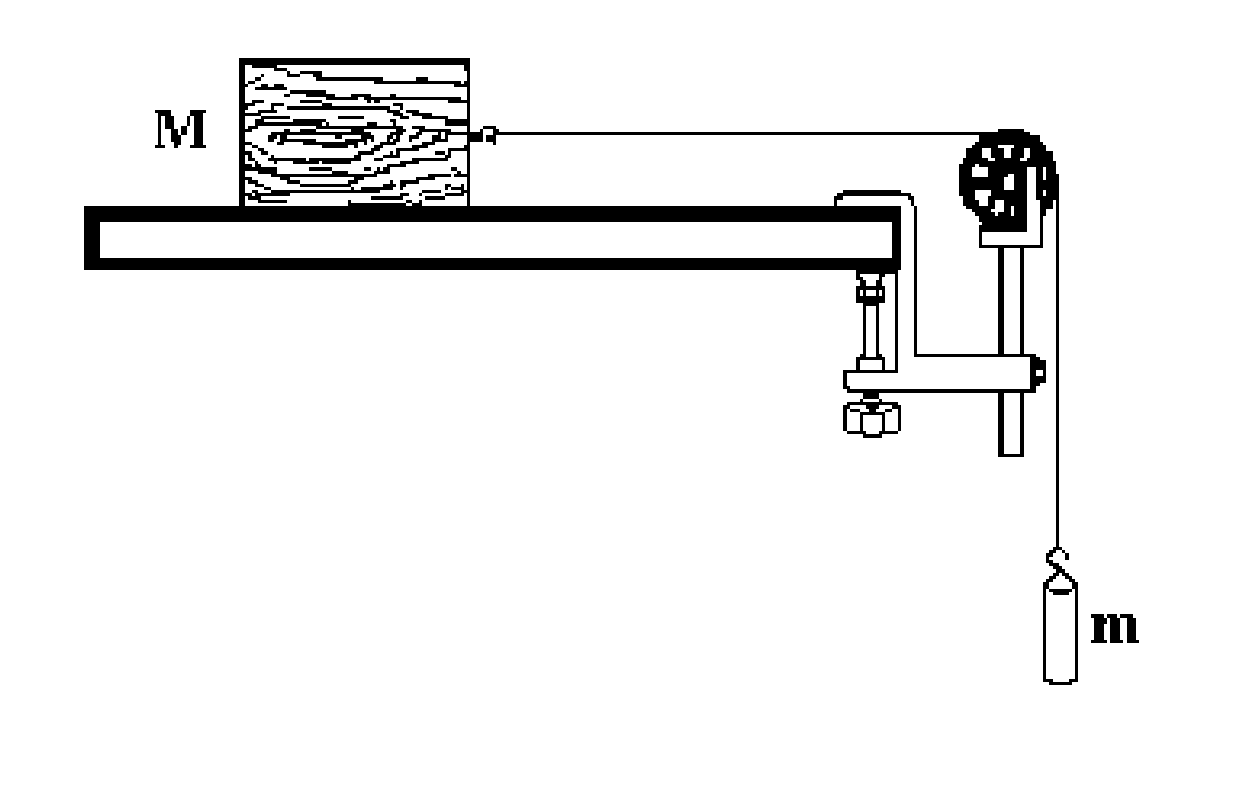
\includegraphics{kineticD.eps}}}}
\end{center}
% \vspace{3.5in}
%   \special{bmp:kinetic.bmp x=4.5in y=3in}
 \caption{Kinetic Friction Apparatus  \label{fig:kinetic}}
\end{figure}
The Smart Pulley should be connected to Digital Channel 1 on the Pasco interface box.
This device reads position by scanning the pulley spokes with a beam
of light.  It thus measures the angular velocity of the pulley.  The
computer uses the radius to convert angular velocity to the linear
velocity of the edge of the pulley---that velocity is of course equal
to the velocity of the descending mass.

\section*{Procedure}
Set up the apparatus as shown in the Figure, plug in your Smart
Pulley, and turn on the computer if it isn't already on.  At this
point you're ready to run the {\em Science Workshop} program.  Your TA
will give you specific instructions on the use of this software.

You will be taking a number of sets of data.  For each set, use the
procedure outlined below:

\begin{enumerate}
%
\item Place enough mass on the hanger so that the block will slide
on the table without needing an initial push (since we are measuring
{\em kinetic} friction).
%
\item Pull the block back until the mass $m$ is raised to the pulley.
Hold the block at rest until the next step.   Be sure that the string
is level.
%
\item  When the computer is ready to take data, release the block.
%
\item Now you can view the velocity vs.\ time data on a
Scientific Workshop graph.  Transfer the linear portion of these data
to the Linfit spreadsheet, and do a least-squares fit to find
the slope (that is, the acceleration).  You don't need to print the
fit report, but do record the acceleration in your spreadsheet or notebook.
(Recall: $\delta v = .003\; {\rm m/s}$.)
%
\item For each mass $m$, do four separate runs, and find the
acceleration for each.  

Find the average acceleration and determine
its error using the standard deviation of the mean. Compare the
Linfit reported errors in $a$ to the error in $a$ determined from
the standard deviation of the mean.  Are these error estimates
in the same ballpark (say within a factor of 2)? We will
use these results to find a value for $\mu_k$ (and its error)
for each mass $m$.  It may be convenient to save
your data in a single spreadsheet file, with a separate worksheet page
for each $m$.
%
\item Repeat the above procedure at least three or four times, each
time for a {\em different} mass $m$, keeping everything else constant.
For
each $m$, take data from four runs.  Choose your values of $m$ to get
as wide a range of accelerations as possible---that way, we will be
measuring $\mu_k$ under a wide range of experimental conditions.
%
\end{enumerate}

\section*{Data Reduction and Analysis}

For each $m$, calculate four values for $\mu_{k}$ using Eq.~\ref{eq:kinfric}  
using the four accelerations you have already found.  Then, find the average value.

Find the uncertainty in $\mu_{k}$ by calculating the standard deviation
of the mean, as discussed in the Reaction Time experiment on page \pageref{exp:react}.
This calculation may be done easily using a spreadsheet.  Note, however, that 
this method does not take into account uncertainties in the masses, so be
sure those measurements are as accurate as possible.  

We use this method 
because a calculation of the uncertainty in
$\mu_{k}$ using the methods of Appendix A is fairly involved. 

%Find the error in this $\mu_{k}$ using the ``high-low game". 
%(Note the maximum value of $\mu_{k}$ is achieved with:
%$M^-$, $a^-$, and $m^+$.)
%
%This  crude method has
%the advantage of simplicity but it
%neglects canceling errors.

Make a final results table including $m$, $a$, $\mu_{k}$, and
the uncertainty in $\mu_{k}$.  
Somewhere in the table note the mass of the sliding block ($M$).

You will find that the velocity vs.\ time plots are not exactly
linear.  Often there will be a kink where the slope (acceleration)
changes appreciably.  Select such a data set and print out a copy of 
the graph (with fit line).  What do you think caused this behavior?

\section*{More experiments}

Do as many of the following additional experiments as time permits.

\begin{enumerate}
\item Make another table of $M$, $\mu_{k}$, and $a$ (different
mass $M$ this time).
Try to do four trials, varying the mass $M$ of
the block each time, but holding the hanging mass $m$ constant.
You can change $M$ by setting masses on the block, but be sure you
start with enough mass $m$ on the hanger that it will always slide.
In calculating the error in $\mu_{k}$,
use the Linfit reported error in $a$ rather than the standard deviation
of the mean (since you will be doing just one trial for every
$M$ value).
%
\item  Use masses from your first data set and compare what happens
if you slide the block {\em on its side}.  (Remember to adjust the
pulley height so the string is level!) This experiment will test
whether surface area effects
the kinetic friction coefficient.  Note results in your lab book, comparing the two sets
of data.
%
\item Try to get an estimate of the \underline{static} coefficient of friction
$\mu_{s}$ using the materials provided.
Is it higher or lower than $\mu_{k}$?  Record your results with error.
{\em (Note: you won't need the computer for this part---it's a
simple, but rough, estimate)}
%
%\item Calculate the error in $\mu_{k}$ using the values given by your TA for error in $a$, $m$
%and $M$.  Then compare this to the standard deviation of the mean of your values for $\mu_{k}$
%\item Summarize your results, answer the questions below, and turn in your notebook.
\end{enumerate}

\section*{Conclusions}
Consider your data, including uncertainties, and discuss the
following questions carefully and in detail:

Did the coefficient of friction vary
with speed?
With acceleration? With surface area? With the mass of the block?

Overall, how good is our assumption that the coefficient of kinetic
friction is constant, within the limits of experimental error?


\section*{Critique of Lab}
     Follow the suggestions given in the Introduction to the
Laboratory Manual.

%\newpage
%\cleardoublepage
%\begin{center}
% CHECKLIST - Kinetic Friction \\
%\end{center}
%\bigskip
%\begin{center}
%\begin{tabular}{||l|r||}
%ASPECT CONSIDERED & DONE? \\ \hline
%Prelab experiment and proof & \\ \hline
%Table of $m$, $a$, $R$, and $\mu_{k}$ with units and uncertainties & \\ \hline
%Table of $M$, $a$, $R$, and $\mu_{k}$ with units and uncertainties & \\ \hline
%Evaluation of surface area data & \\ \hline
%Summary of results & \\ \hline
%Calculated uncertainties $\delta \mu_{k}$, Compare to $\sigma_{\bar x}$ & \\ %\hline
%Questions answered & \\ \hline
%Cleanup & \\ \hline
%\end{tabular}
%\end{center}
\bigskip
\bigskip
\bigskip

%%COMMENTS:\\
%\newpage
%\newpage
%\bigskip
%\begin{center}
%{\bf Pre-Lab}
%\end{center}
%\centerbmp {4in}{2in}{coin.bmp}
%Perform the following
%mini-experiment: Get a book, a coin, and a ruler.  Place a coin on your closed book.
%Now tilt the book until the coin begins to slide, then lower it until it slides
%down the book at a constant speed. Note this position, then measure
% the angle $\theta$ the book is tilted (by measuring
%two sides of the ``triangle'').  Now calculate the friction coefficient,using
%$\tan \theta = \mu$ and record
% your results.  Question: Is the $\mu$ you just found the Kinetic or Static friction coefficient?  Derive the equation $\tan \theta = \mu$ starting with Newton's Second Law.
%
% {\em Hint: Sum the forces on the coin in the x direction (parallel to the table top), finding the components of N and the frictional
%force.  Then substitute the definition of the frictional force and solve for
%$\mu$.}
%\bigskip
